\subsection{Tipo de entidad Titulación}

   \begin{description}

   \item[Definición] Se refiere al objeto del mundo real: \emph{``Conjunto de
        materias cuya superación supone la obtención de un título académico''}.

   \item[Características] La entidad presenta las siguientes características:
      \begin{itemize}
         \item \textbf{Nombre:} Titulación.
         \item \textbf{Tipo:} Débil por identificación con respecto a Centro.
         \item \textbf{Número de atributos:} 4.
         \item \textbf{Atributo/s identificador/es principal/es:} id\_centro junto con \\id\_titulación.
         \item \textbf{Atributo/s identificador/es alternativo/s:} id\_centro junto con nombre\_titulación y plan\_estudios.
         \item \textbf{Atributo/s heredado/s:} id\_centro del tipo de entidad Centro.
      \end{itemize}

   \item[Diagrama]
   \item \begin{figure}[h!]
            \begin{center}
            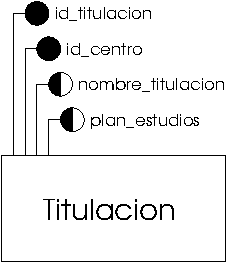
\includegraphics[]{07.Modelo_Entidad-Interrelacion/7.2.Analisis_Entidades/diagramas/titulacion.pdf}
            \caption{Diagrama de la entidad Titulación.}
            \end{center}
         \end{figure}

   \item[Descripción de los atributos] La entidad presenta los siguientes
   atributos:

   \begin{itemize}
   \item \textbf{id\_centro}
      \begin{itemize}
         \item \textbf{Definición:} Código que sirve como número identificativo
               para cada centro del sistema.
         \item \textbf{Dominio:} Números naturales.
         \item \textbf{Carácter:} Obligatorio.
         \item \textbf{Ejemplo práctico:} 15.
         \item \textbf{Información adicional:} El dato se hereda del tipo de
         entidad Centro. Es la clave primaria junto con id\_titulación. También
         actúa de clave alterna junto con nombre\_titulación y plan\_estudios.
      \end{itemize}
   \item \textbf{id\_titulacion}
      \begin{itemize}
         \item \textbf{Definición:} Código que sirve como número identificativo
         para cada titulación dentro del sistema.
         \item \textbf{Dominio:} Números naturales.
         \item \textbf{Carácter:} Obligatorio.
         \item \textbf{Ejemplo práctico:} 3.
         \item \textbf{Información adicional:} El dato lo genera el sistema
         cuando el administrador, principal o de centro, introduce la titulación
         en el sistema. Es la clave primaria junto con id\_centro.
      \end{itemize}
   \item \textbf{nombre\_titulación}
      \begin{itemize}
         \item \textbf{Definición:} Denominación de una titulación dentro del sistema.
         \item \textbf{Dominio:} Conjunto de caracteres alfanuméricos.
         \item \textbf{Carácter:} Obligatorio.
         \item \textbf{Ejemplo práctico:} Ingeniería Técnica en Informática de Gestión.
         \item \textbf{Información adicional:} El dato lo proporciona el administrador, principal o de centro, en el momento de introducir la titulación en el sistema. Es la clave alterna junto con id\_centro y con plan\_estudios.
      \end{itemize}
   \item \textbf{plan\_estudios}
      \begin{itemize}
         \item \textbf{Definición:} Especifica el año del plan de estudios de la titulación.
         \item \textbf{Dominio:} Formato de fecha: aaaa.
         \item \textbf{Carácter:}  Obligatorio
         \item \textbf{Ejemplo práctico:} 1999
         \item \textbf{Información adicional:} El dato lo proporciona el administrador, principal o de
         centro, en el momento de introducir la titulación en el sistema. Es la clave alterna junto con
         id\_centro y nombre\_titulación.
      \end{itemize}
   \end{itemize}

   \item[Ejemplo práctico]

   \item \begin{center}
            \begin{tabular}{ | l | l | }
            \hline
            \multicolumn{2}{ | c | }{\textbf{Tipo de entidad Titulación}} \\
            \hline
            id\_centro & 15 \\
            \hline
            id\_titulación & 3\\
            \hline
            nombre\_titulación & Ingeniería Técnica en Informática de Gestión \\
            \hline
            plan\_estudios & 1999\\
            \hline
            \end{tabular}
         \end{center}
   \end{description}
